\documentclass[a4paper]{article}

\usepackage[utf8]{inputenc}
\usepackage[portuguese]{babel}
\usepackage{a4wide}
\usepackage[pdftex]{hyperref}
\usepackage{graphicx}
\usepackage{wrapfig}
\usepackage{amsmath}
\usepackage{caption}
\usepackage{subcaption}
\usepackage{tikz}
\usepackage{pgfplots}
\pgfplotsset{compat=1.10}
\usepgfplotslibrary{fillbetween}
\usepackage{pgfplots}
\usetikzlibrary{patterns}
\usepackage{float}



\begin{document}

\begin{titlepage}
\begin{center}



\includegraphics[width=0.4\textwidth]{logo}\\[0.3cm]

{\large Universidade do Minho - Escola de Engenharia}\\[0.5cm]

{\large Relatório do trabalho prático de Desenvolvimento de Sistemas de Software}\\[0.5cm]



% Title
\rule{\linewidth}{0.5mm} \\[0.4cm]
{ \huge \bfseries Sistema de Gestão de Turnos Práticos \\[0.4cm] }
\rule{\linewidth}{0.5mm} \\[1.5cm]

% Author and supervisor
\noindent
\begin{minipage}{0.4\textwidth}
  \begin{flushleft} \large
    \emph{Autores :}\\
    Diana Costa \textsc{(A78985)}\\
    
\includegraphics[width=1.5cm]{diana}\break
    Marcos Pereira \textsc{(A79116)}\\
    
\includegraphics[width=1.5cm]{marcos}\break
    Sérgio Oliveira\textsc{(A77730)}\\
    
\includegraphics[width=1.5cm]{sergio}\break
    Vitor Castro\textsc{(A77870)}\\
    
\includegraphics[width=1.5cm]{vitor}\break
  \end{flushleft}
\end{minipage}%
\vfill

% Bottom of the page
{\large Versão 1.0 \\ \today}

\end{center}
\end{titlepage}


\begin{abstract}

\hspace{3mm}Neste relatório será feita uma abordagem inicial ao projeto de Desenvolvimento de Sistemas de Software ao qual está associado o desenvolvimento de um programa, em Java, responsável pela gestão dos turnos de um curso. Assim, este documento apresenta, detalhadamente, a perspetiva tomada pelo grupo em relação ao problema proposto pela equipa docente de DSS.

\end{abstract}

\pagebreak
\tableofcontents

\pagebreak
\section{Introdução}
\label{sec:1}

\hspace{3mm}Este projeto tem como objetivo desenvolver um sistema capaz de alocar e gerir os turnos de um curso. A sua execução permitirá consolidar conhecimentos ao nível da programação em linguagens de objetos e introduz abordagens organizadas e estruturadas de desenvolvimento de software a partir de modelação e representação de dados em \emph{UML 2.x}. 
Nesta fase intermédia do trabalho foi então sugerida a concepção da representação gráfica ou diagramas nessa linguagem.

\section{Problema}
\label{sec:2}

\hspace{3mm}

\hspace{3mm}Pretende-se desenvolver um sistema que atribui turnos (e, deste modo, um horário) aos alunos do curso e possibilita a ocorrência de trocas entre estes. As trocas estão condicionadas pela existência de dois alunos interessados em trocar de turno, no caso de pertencerem ao regime normal, e são feitas sem condicionalismos no caso do aluno ser trabalhador estudante.
Neste momento, deve apresentar-se uma análise de requisitos da qual resultará um Modelo de Domínio, um Modelo de Use Case e uma proposta de interface gráfica.

\section{Solução}
\label{sec:3}


\hspace{3mm}A solução apresentada baseia-se na UML - emph{Unified Modeling Language} - linguagem útil na elaboração, modelação e documentação da estrutura de projetos de software e de sistemas orientados a objetos. Portanto, auxilia os \emph{developers} de programas a visualizarem os seus sistemas através de diagramas padronizados.
Até ao momento, a solução foi implementada com base em:

\begin{itemize}
    \item Esquema de Domínio;
    \item Esquema de Use Case;
    \item Especificação dos Use Case;
    \item Proposta para a Interface Gráfica
\end{itemize}

\pagebreak
\subsection{Esquema de Domínio}
\hspace{3mm}O modelo de domínio analisa o problema de uma perspetiva concetual e é uma aproximação da representação gráfica das classes do programa e dos seus atributos, assim como o relacionamento entre estas.


\begin{figure}[h!]
\centering
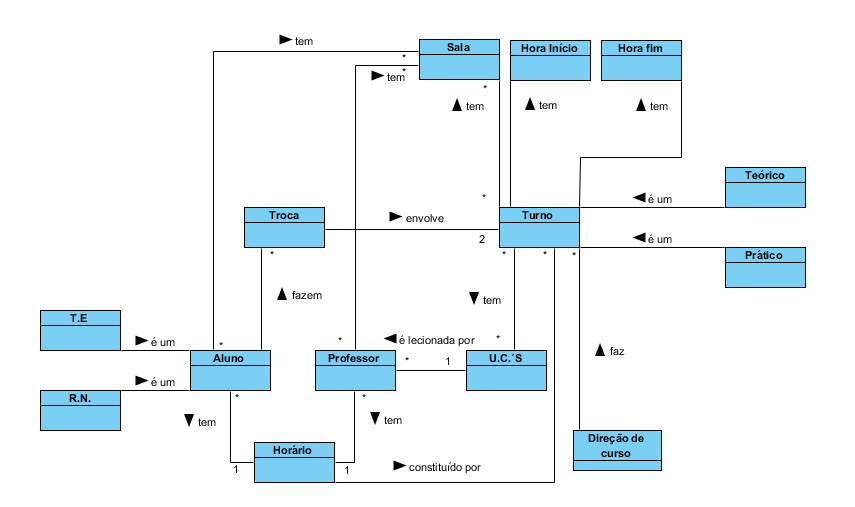
\includegraphics[width=12cm]{dominio}
\caption{Modelo de Domínio proposto.}
\label{fig:1}
\end{figure}


\subsection{Esquema de Use Case}

\hspace{3mm}O esquema de Use Cases é o diagrama que mostra o que o programa faz do ponto de vista do utilizador, ou seja, consegue mostrar as principais funcionalidades do sistema e as suas interações com os atores do mesmo. Por isso, os diagramas de use case são compostos por atores (utilizadores do sistema), por use cases (funcionalidade) e pelas comunicações entre atores e use case.
O grupo equacionou várias hipóteses para que fosse possível representar interações de utilizadores idênticos (como Trabalhador-estudante e Aluno, ou Docente-Responsável e Docente), e o resultado encontra-se na figura~\ref{fig:2}. Relativamente ao primeiro tuplo (Trabalhador-estudante e Aluno), decidiu-se pela unificação em Aluno, uma vez que o sistema será baseado numa bolsa de trocas, contrariamente ao plano inicial, que seria cada aluno propôr a troca a um outro (tal como desenvolvido no sistema SWAP em vigor). Com esta bolsa de trocas, todos os alunos (trabalhadores-estudantes ou não) teriam igualdade de oportunidade de troca, tendo sido assumido que, caso houvesse um trabalhador-estudante com problemas de turnos, este contactaria diretamente a DC (tal como acontece na realidade), dispensando-se essa responsabilidade do programa. No que toca ao segundo tuplo (Docente-Responsável e Docente), depois de refletir sobre a pertinência de haver uma entidade Docente (que não responsável da UC) e sabendo que a única interação que poderia ter seria a de registar faltas, decidiu-se pela sua retirada. O motivo desta decisão prende-se pelo objetivo da Plataforma a ser desenvolvida, a saber, resolver um problema de atribuição de horários, e não pela marcação de faltas (apesar das mesmas terem uma implicação no horário de um Aluno, caso este falte a mais de 25 por cento das aulas). Deste modo, assume-se que as faltas serão contabilizadas tal como o são no momento e, a dada altura, o Docente-Responsável aperceber-se-á que determinado aluno deve ser removido do turno, funcionalidade essa que está disponível.

A Direção de Curso foi criada com o objetivo de poder ser o controlador principal de todo o sistema, sendo que pode fazer qualquer operação sem problema (mesmo que implique, a título de exemplo, inscrever um Aluno num turno que já está cheio). Tendo este caráter, qualquer problema de compatibilidade operado por este interveniente não será da responsabilidade de verificação do programa.


\begin{figure}[h!]
\centering
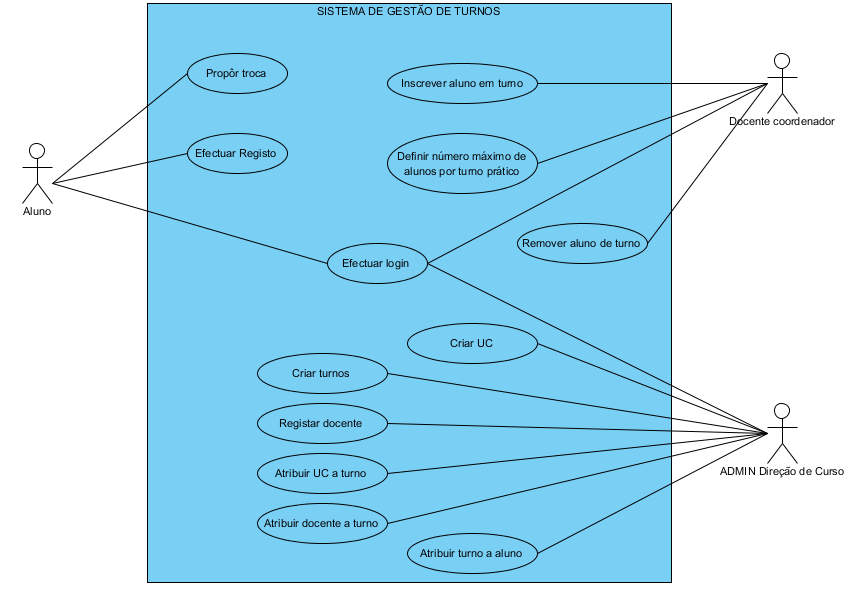
\includegraphics[width=12cm]{diagramausecase}
\caption{Diagrama de Use Cases proposto.}
\label{fig:2}
\end{figure}




\subsection{Especificação textual dos Use Case}
\hspace{3mm}Dado que um cenário é uma sequência de passos da interação entre ator e sistema, então a especificação textual dos casos de uso é um documento que descreve os vários cenários possíveis entre as comunicações de um mesmo objetivo ou funcionalidade. Apenas serão explicados alguns dos Use Cases (considerados mais importantes), uma vez que a sua explanação é suficiente para a compreensão de todo o problema.

\subsubsection{Atribuir docente a turno}

\begin{figure}[H]
\centering
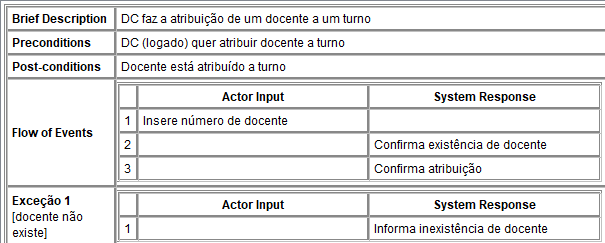
\includegraphics[width=12cm]{atribuidocenteturno}
\caption{}
\label{fig:3}
\end{figure}


\subsubsection{Atribuir turno a aluno}

\begin{figure}[H]
\centering
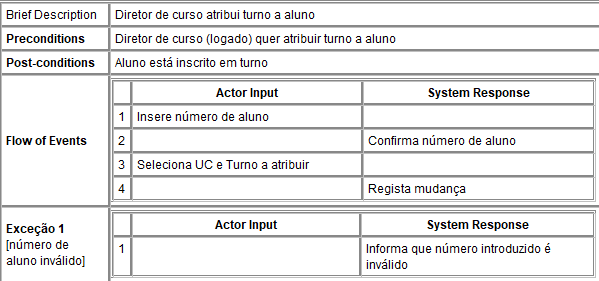
\includegraphics[width=12cm]{atribuiturnoaluno}
\caption{}
\label{fig:4}
\end{figure}


\subsubsection{Atribuir UC a turno}
\hspace{3mm}Responsabilidade do DC, que poderá atribuir a um turno a correspondente UC. O sistema apenas verifica a existência do turno e UC especificados, registando a atribuição.

\begin{figure}[H]
\centering
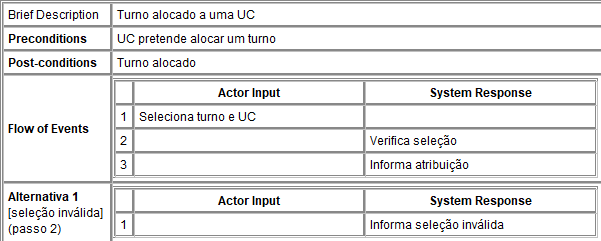
\includegraphics[width=12cm]{atribuiucaturno}
\caption{}
\label{fig:5}
\end{figure}


\subsubsection{Registar docente}

\begin{figure}[H]
\centering
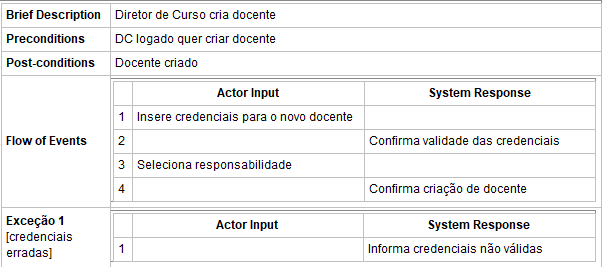
\includegraphics[width=12cm]{registardocente}
\caption{}
\label{fig:6}
\end{figure}


\subsubsection{Criar turnos}

\begin{figure}[H]
\centering
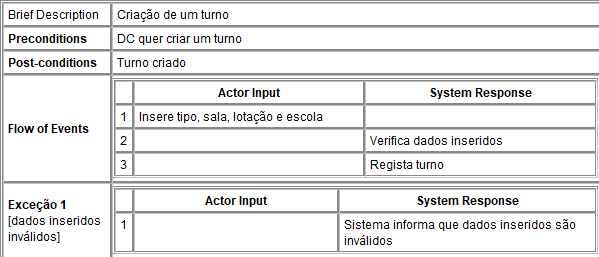
\includegraphics[width=12cm]{criarturnos}
\caption{}
\label{fig:7}
\end{figure}


\subsubsection{Criar UC}
\hspace{3mm}Responsabilidade do DC, que deve inserir a UC no sistema, preenchendo os campos necessários à caracterização da mesma. O sistema verifica a inserção dos dados e cria a UC, caso tudo esteja correto.


\begin{figure}[H]
\centering
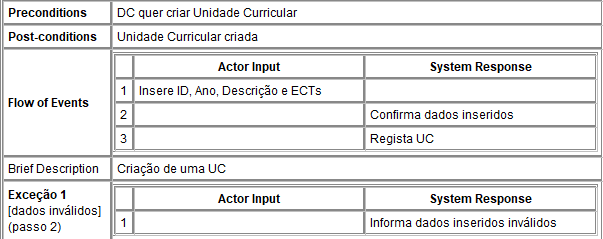
\includegraphics[width=12cm]{criaruc}
\caption{}
\label{fig:8}
\end{figure}


\subsubsection{Efectuar Login}
\hspace{3mm}O utilizador (Aluno, Docente ou DC) faz login. As suas credenciais são verificadas e, caso aprovadas, terá acesso à sua área pessoal de acordo com os seus privilégios. O login é negado caso o utilizador seja inexistente ou a password não seja a correta.

\begin{figure}[H]
\centering
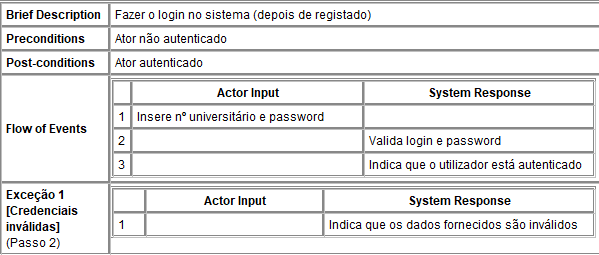
\includegraphics[width=12cm]{efectuarlogin}
\caption{}
\label{fig:9}
\end{figure}


\subsubsection{Remover aluno de turno}
\hspace{3mm}Responsabilidade atribuída ao Docente-Responsável, que apenas terá de indicar o aluno que quer remover e. O sistema verifica a existência do aluno e será responsável pela identificação do turno onde aquele aluno está inscrito, removendo-o.

\begin{figure}[H]
\centering
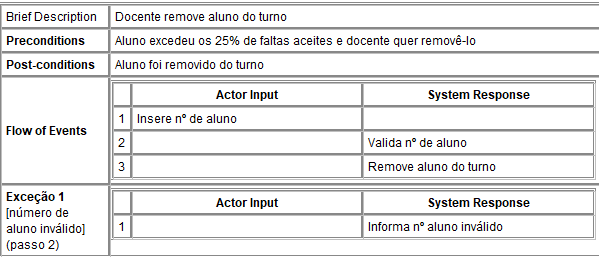
\includegraphics[width=12cm]{removeralunoturno}
\caption{}
\label{fig:10}
\end{figure}
\pagebreak

\subsubsection{Definir número máximo de alunos por turno prático}
\hspace{3mm}Responsabilidade atribuída ao Docente-Responsável, que poderá definir um número de alunos máximo dentro dos intervalo 0 até CAPACIDADE DA SALA, sendo esta a única verificação feita pelo sistema. No fim, o número será definido.

\begin{figure}[H]
\centering
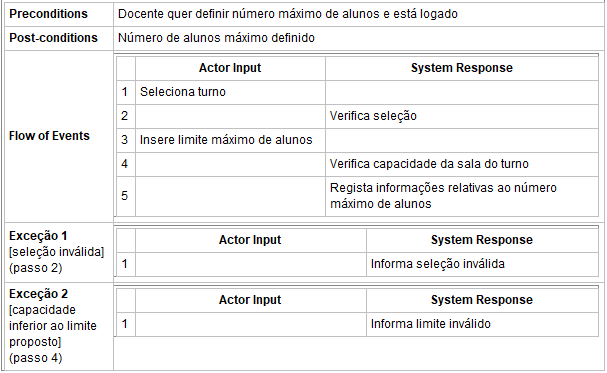
\includegraphics[width=12cm]{definiralunos}
\caption{}
\label{fig:11}
\end{figure}


\subsubsection{Inscreve aluno em turno}
\hspace{3mm}Tarefa atribuída ao Docente-Responsável que, segundo uma política de utilização responsável, não terá qualquer problema em adicionar qualquer aluno ao turno desejado (da UC que leciona), mesmo que aquele esteja cheio. Apenas se verifica a existência daquele aluno no sistema.

\begin{figure}[H]
\centering
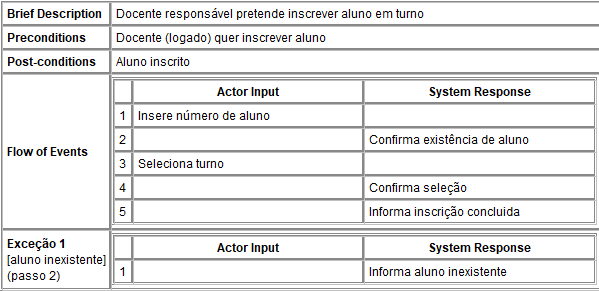
\includegraphics[width=12cm]{inscreveralunoturno}
\caption{}
\label{fig:12}
\end{figure}

\pagebreak
\subsubsection{Efectuar Registo}
\hspace{3mm}Só efetuado por alunos que, durante o registo, escolherão o seu regime e também as UCs a que se querem inscrever. É feita a verificação de inserção dos dados.

\begin{figure}[H]
\centering
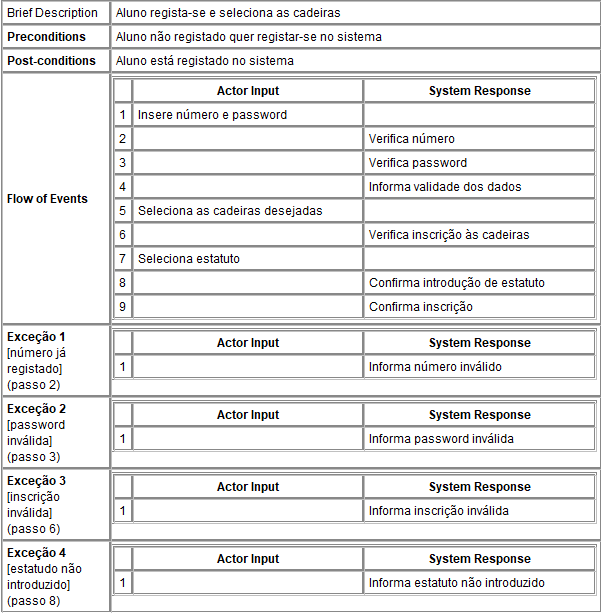
\includegraphics[width=12cm]{efectuarregisto}
\caption{}
\label{fig:13}
\end{figure}


\subsubsection{Propôr Troca}
\hspace{3mm}Só efetuado por alunos sendo que, após seleção do turno e UC desejados, é lançada essa proposta para a bolsa de trocas. Posteriormente (e não sendo visível ao utilizador), o sistema verificará se existem propostas com reciprocidade, efetuando a troca automaticamente. Apenas é verificada a seleção de UC e turnos.

\begin{figure}[H]
\centering
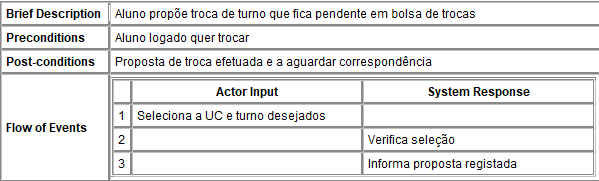
\includegraphics[width=12cm]{proportroca}
\caption{}
\label{fig:14}
\end{figure}



\subsection{Interface Gráfica}
\hspace{3mm} Segue-se a de prototipagem simples da interface, que poderá ser alterada subtilmente, conforme pequenos ajustes do programa a desenvolver. 


\subsubsection{Login/Registo}
\begin{figure}[H]
\centering
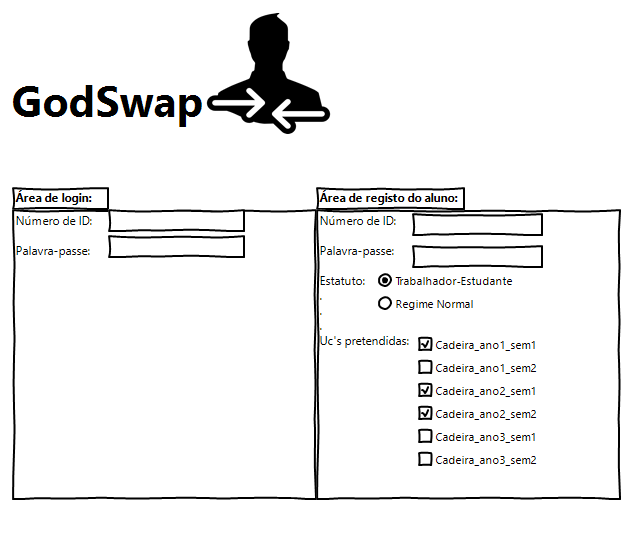
\includegraphics[width=14cm]{interface_1}
\caption{Página inicial da interface e área de registo.}
\label{fig:15}
\end{figure}



\subsubsection{Minha Área}
\begin{figure}[H]
\centering
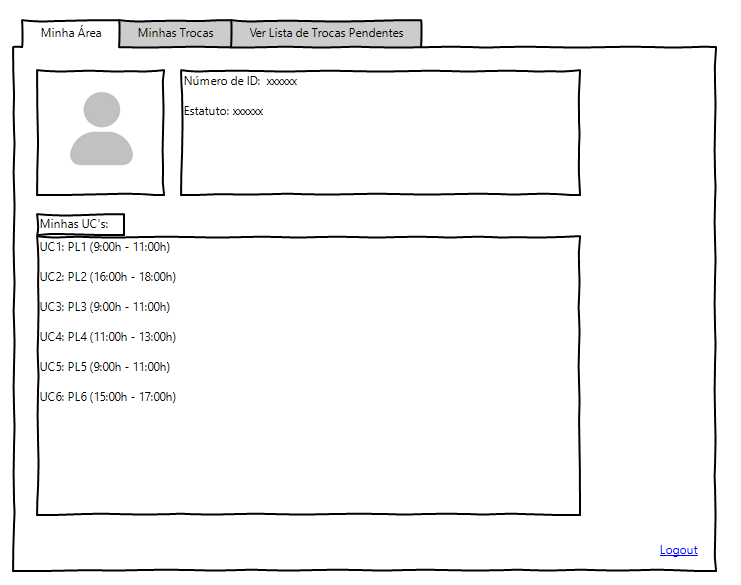
\includegraphics[width=14cm]{interface_2}
\caption{Área pessoal do utilizador em questão.}
\label{fig:16}
\end{figure}


\subsubsection{Minhas Trocas}
\begin{figure}[H]
\centering
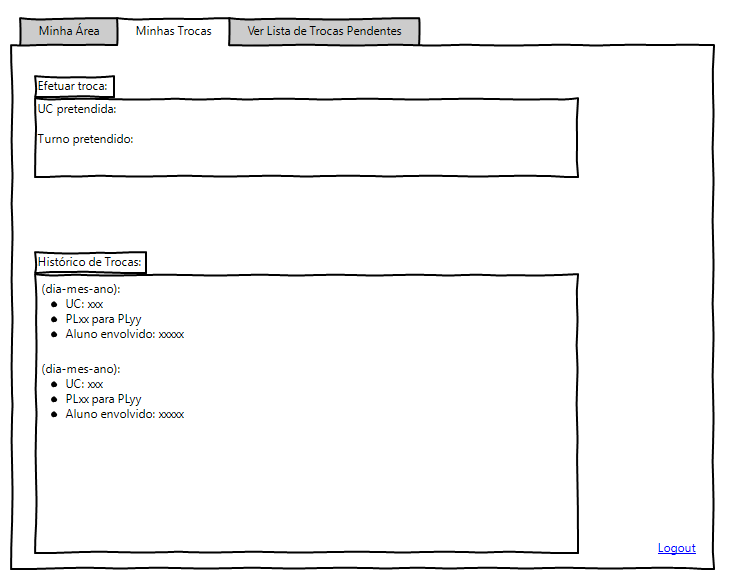
\includegraphics[width=14cm]{interface_3}
\caption{Histórico de trocas efetuadas e dados pessoais.}
\label{fig:17}
\end{figure}

\subsubsection{Ver Lista de Trocas Pendentes}
\begin{figure}[H]
\centering
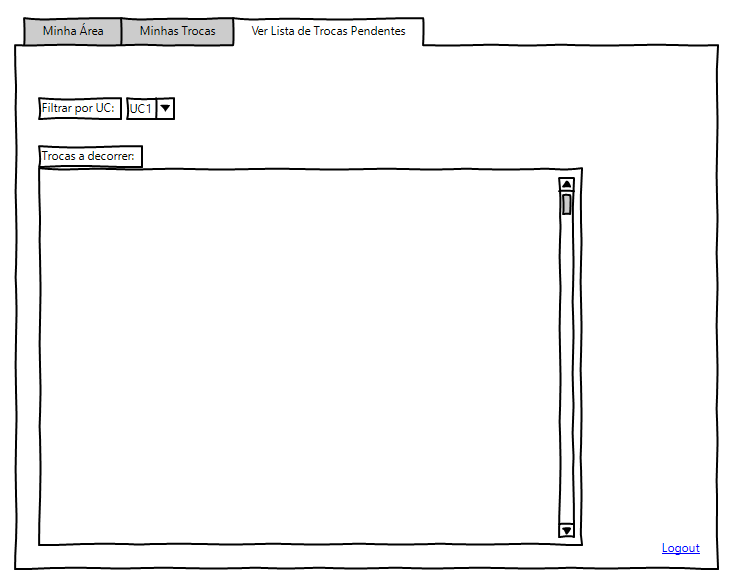
\includegraphics[width=14cm]{interface_4}
\caption{Lista de trocas requeridas por alunos e ainda pendentes.}
\label{fig:18}
\end{figure}



\pagebreak
\section{Conclusões}
\hspace{3mm}Durante a realização desta parte inicial do projeto, foram encontradas algumas dificuldades, principalmente no que toca à realização do Diagrama de Use Cases. Depois de alguma discussão, a equipa definiu que tipo de implementação o sistema teria (i.e., se as trocas seriam propostas diretas ou em forma de bolsa(conjunto)) e, a partir desse momento, tornou-se mais fácil o processo de elaboração dos Use Cases e de definição dos Atores do sistema. Este processo foi importante pois permitiu a consciencialização das implicações que a escolha de determinados Use Cases teria no sistema, sendo que o grupo está confiante na elaboração do software correspondente, tendo consciência que outros dificuldades poderão surgir e que, eventualmente, faça sentido alterar o Diagrama.
\label{sec:4}

\hspace{3mm}
\end{document}
